%!suppress=Unicode
\documentclass{article}[12pt,a4paper]
\usepackage[utf8]{inputenc}
\usepackage{caption}
\usepackage{amsmath}
\usepackage{hyperref}
\usepackage{csquotes}
\usepackage[T1]{fontenc}
\usepackage{booktabs}
\usepackage{subfiles}
\usepackage{listings}
\usepackage[margin=0.8in]{geometry}

\hypersetup{
    colorlinks=true,
    linkcolor=blue,
    filecolor=magenta,
    urlcolor=cyan,
}

\usepackage{graphicx}
\graphicspath{ {./pngs/} }

\title{Részvénypiac Szimuláció - Specifikáció Skeleton Programhoz}
\author{Rátki Barnabás}
\date{2021.04.13}

\newcommand{\tbs}{\textbackslash}
\newcommand{\tc}{\textasciicircum}

\renewcommand*\contentsname{Tartalomjegyzék}

\begin{document}
    \maketitle

    \tableofcontents

    \section{Feladat}\label{sec:feladat}
    \subfile{sub_spec}

    \section{Pontosított feladatspecifikáció}\label{sec:pontositott-feladatspecifikacio}
    A laborvezetőnek eddig semmilyen változtatási igénye nem merült fel, ezért az munkát az eredeti tervek alapján folytattam.
    A következőkben az implementáció részleteivel fogok foglalkozni.\\

    A feladatban elkészített osztályok mezői és függvényei már megtervezésre kerültek, de mivel egy szimulációs feladatról beszélünk, az összes algoritmus konkrét implementációja nem tervezhető meg előre.
    Mivel ez gyakorlatilag a teljes feladat befejezését igényelné, minden componens belső működése előre nem látható hatásokkal lehet a többi komponens működésére.
    Ez a tulajdonság teszi magát a szimulációt érdekessé.

    A feladat megoldásához nem használok \textbf{STL} tárolókat a szálkezeléshez szükséges \textit{std::mutex} osztályon, és más ehhez kapcsolódó és szükséges primitíveken kívül.
    (Illetve még a \textit{std::function} segéd tipust is esedlegesen alkalmazom de ez nem valódi tároló.)

    \section{Terv}
    Az implementáció két részből áll, egy futtatható standard bemenetetn keresztül irányítható programrészből, ami magát a szimulációt is futtatja (ez a program készült végfelhasználásra), illetve egy test programból ami a fordításnál definiálandó \textit{TEST\_VAR} szimbólum \textit{ETEST}-értékre való beállításával elérhető.
    A testprogram a szükséges tárolókat, segéd osztályok működését teszteli, nem célja a teljes kódlefedettség.
    A program nem könyvtárként való használatra készült, ezért minden hiba amit dob az \textit{std::runtime\_error} osztály példánya.
    
    \subsection{Objektum Terv}

    \subsubsection{Könyvtár - Terv}
    A program egy kisebb sablon könyvtárat tartalmaz, a könyebb fejleszhetőség érdekében.
    A könyvtár ujradefiniáls numerikus tipusokat is, hogy azok könyebben használhatóak legyenek.
    Az alábbiak ezek a definíciók:
    \begin{lstlisting}
    typedef std::size_t usize;
    typedef unsigned int u32;
    typedef uint8_t u8;
    typedef uint16_t u16;
    typedef uint32_t u32;
    typedef uint64_t u64;

    typedef int8_t i8;
    typedef int16_t i16;
    typedef int32_t i32;
    typedef int64_t i64;

    typedef float f32;
    typedef double f64;
    typedef long double f128;
    \end{lstlisting}

    Az itt definiált osztályok definícióját és egymáshoz való függőségeit az alábbi UML diagram ábárzolja:
    \begin{center}
        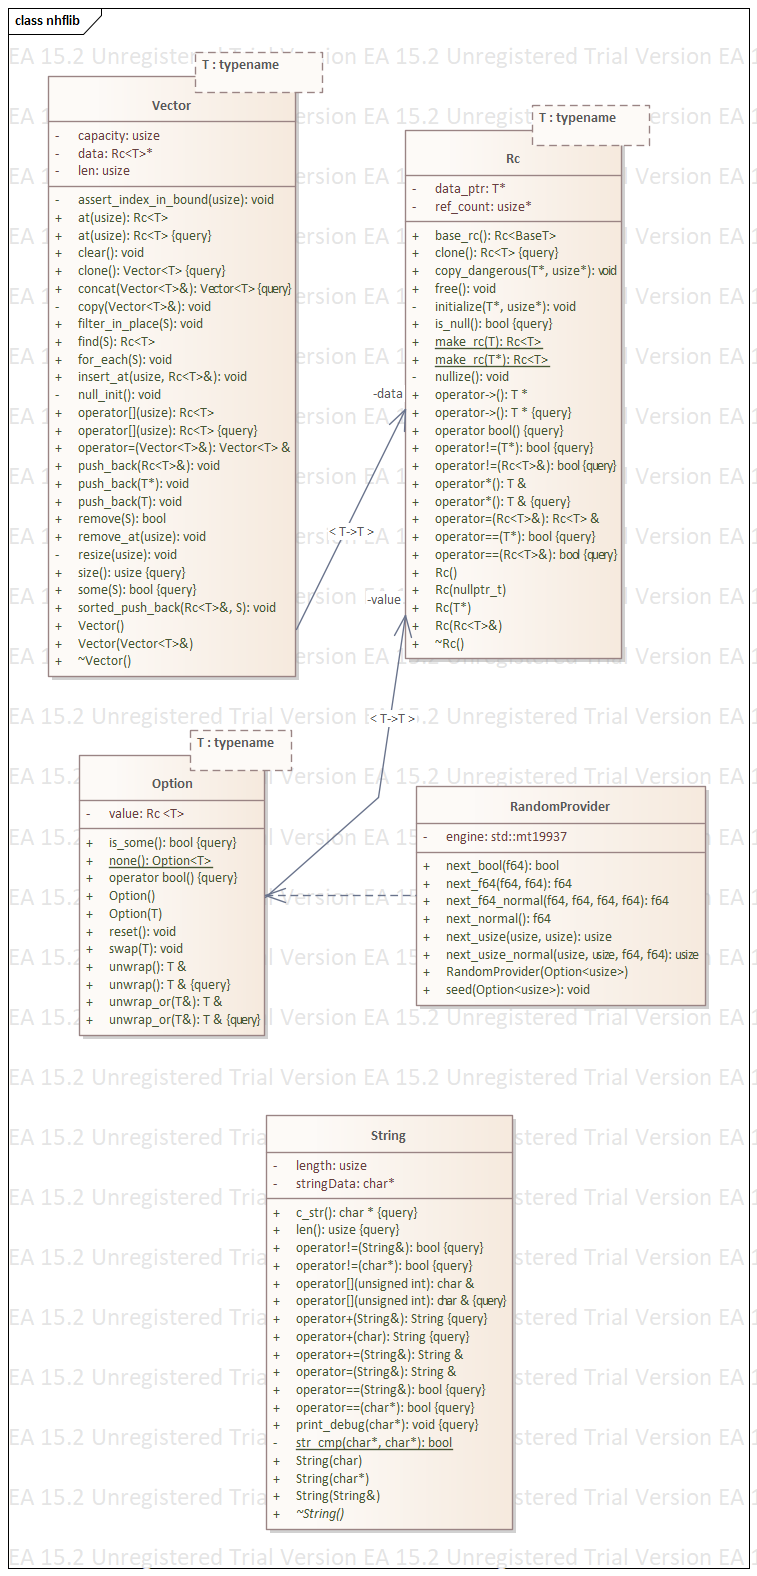
\includegraphics[scale=0.55]{nhflib2}
    \end{center}

    \subsubsection{Rc<T> - Implementáció}
    Egy reference számolt, T tipusu dinamikusan tárolt pointert tartalmaz.
    A reference számolást egy dinamikusan tárolt \textit{usize} pointerrel valósítja meg.
    Egy Rc<T> másolásánál, a reference számláló növelve van eggyel illetve a pointerek másolva vannak.
    Destrukciónál a reference számláló csökkentve van egyel, és a belsőleg tárolt adat csak akkor van felszabadítva ha a reference számláló nulla.

    \subsection{Implementációs - Terv}
    A szimuláció főleg kompozícióval épül fel, a proram a \textit{SimulationCli} osztály példányának létrehozásával és a \textit{start} függvényének meghívásával indul el.
    A szimuláció osztály \textit{run} függvénye egy második szállon fut, és egy mutex segítségével van a futási állapota szinkronizálva a CLI-vel. \\
    Alapvetően a szimulációban lévő kereskedők egy heterogén kollekcióban vannak tárolva, minden osztály ami kompatibilis a \textit{TraderAgent} osztállyal működhet kereskedő "inteligenciaként".
    A cégek egy speciális \textit{TraderAgent} implementáción keresztül adják el az első részvényeiket (IPO szimulácóió amit brókerek kezelnek). \\
    A kereskedők random időközönként aktiválódnak és az \textit{on\_cycle} fügvényük meghívódik, a paraméterként kapott \textit{ExchangeApi}-n keresztül tudnak megnyitni új pozíciókat és információt szerezni a piaci körülményekről a döntéshozáshoz.\\
    Alapvető feltételezés, hogy a \textit{TraderAgent} nem megbízható, tehát ha tud akkor akár csalni is fog, ezért úgy került megtervezésre, hogy a benne futó kódban ne kelljen megbízni.
    Nem dobhat hibákat, és semmilyen "szenzitív" adathoz nem fér hozzá.

    Az osztálydiagram sokkal beszédesebben leírja a különböző kompozíciókat:
    \begin{center}
        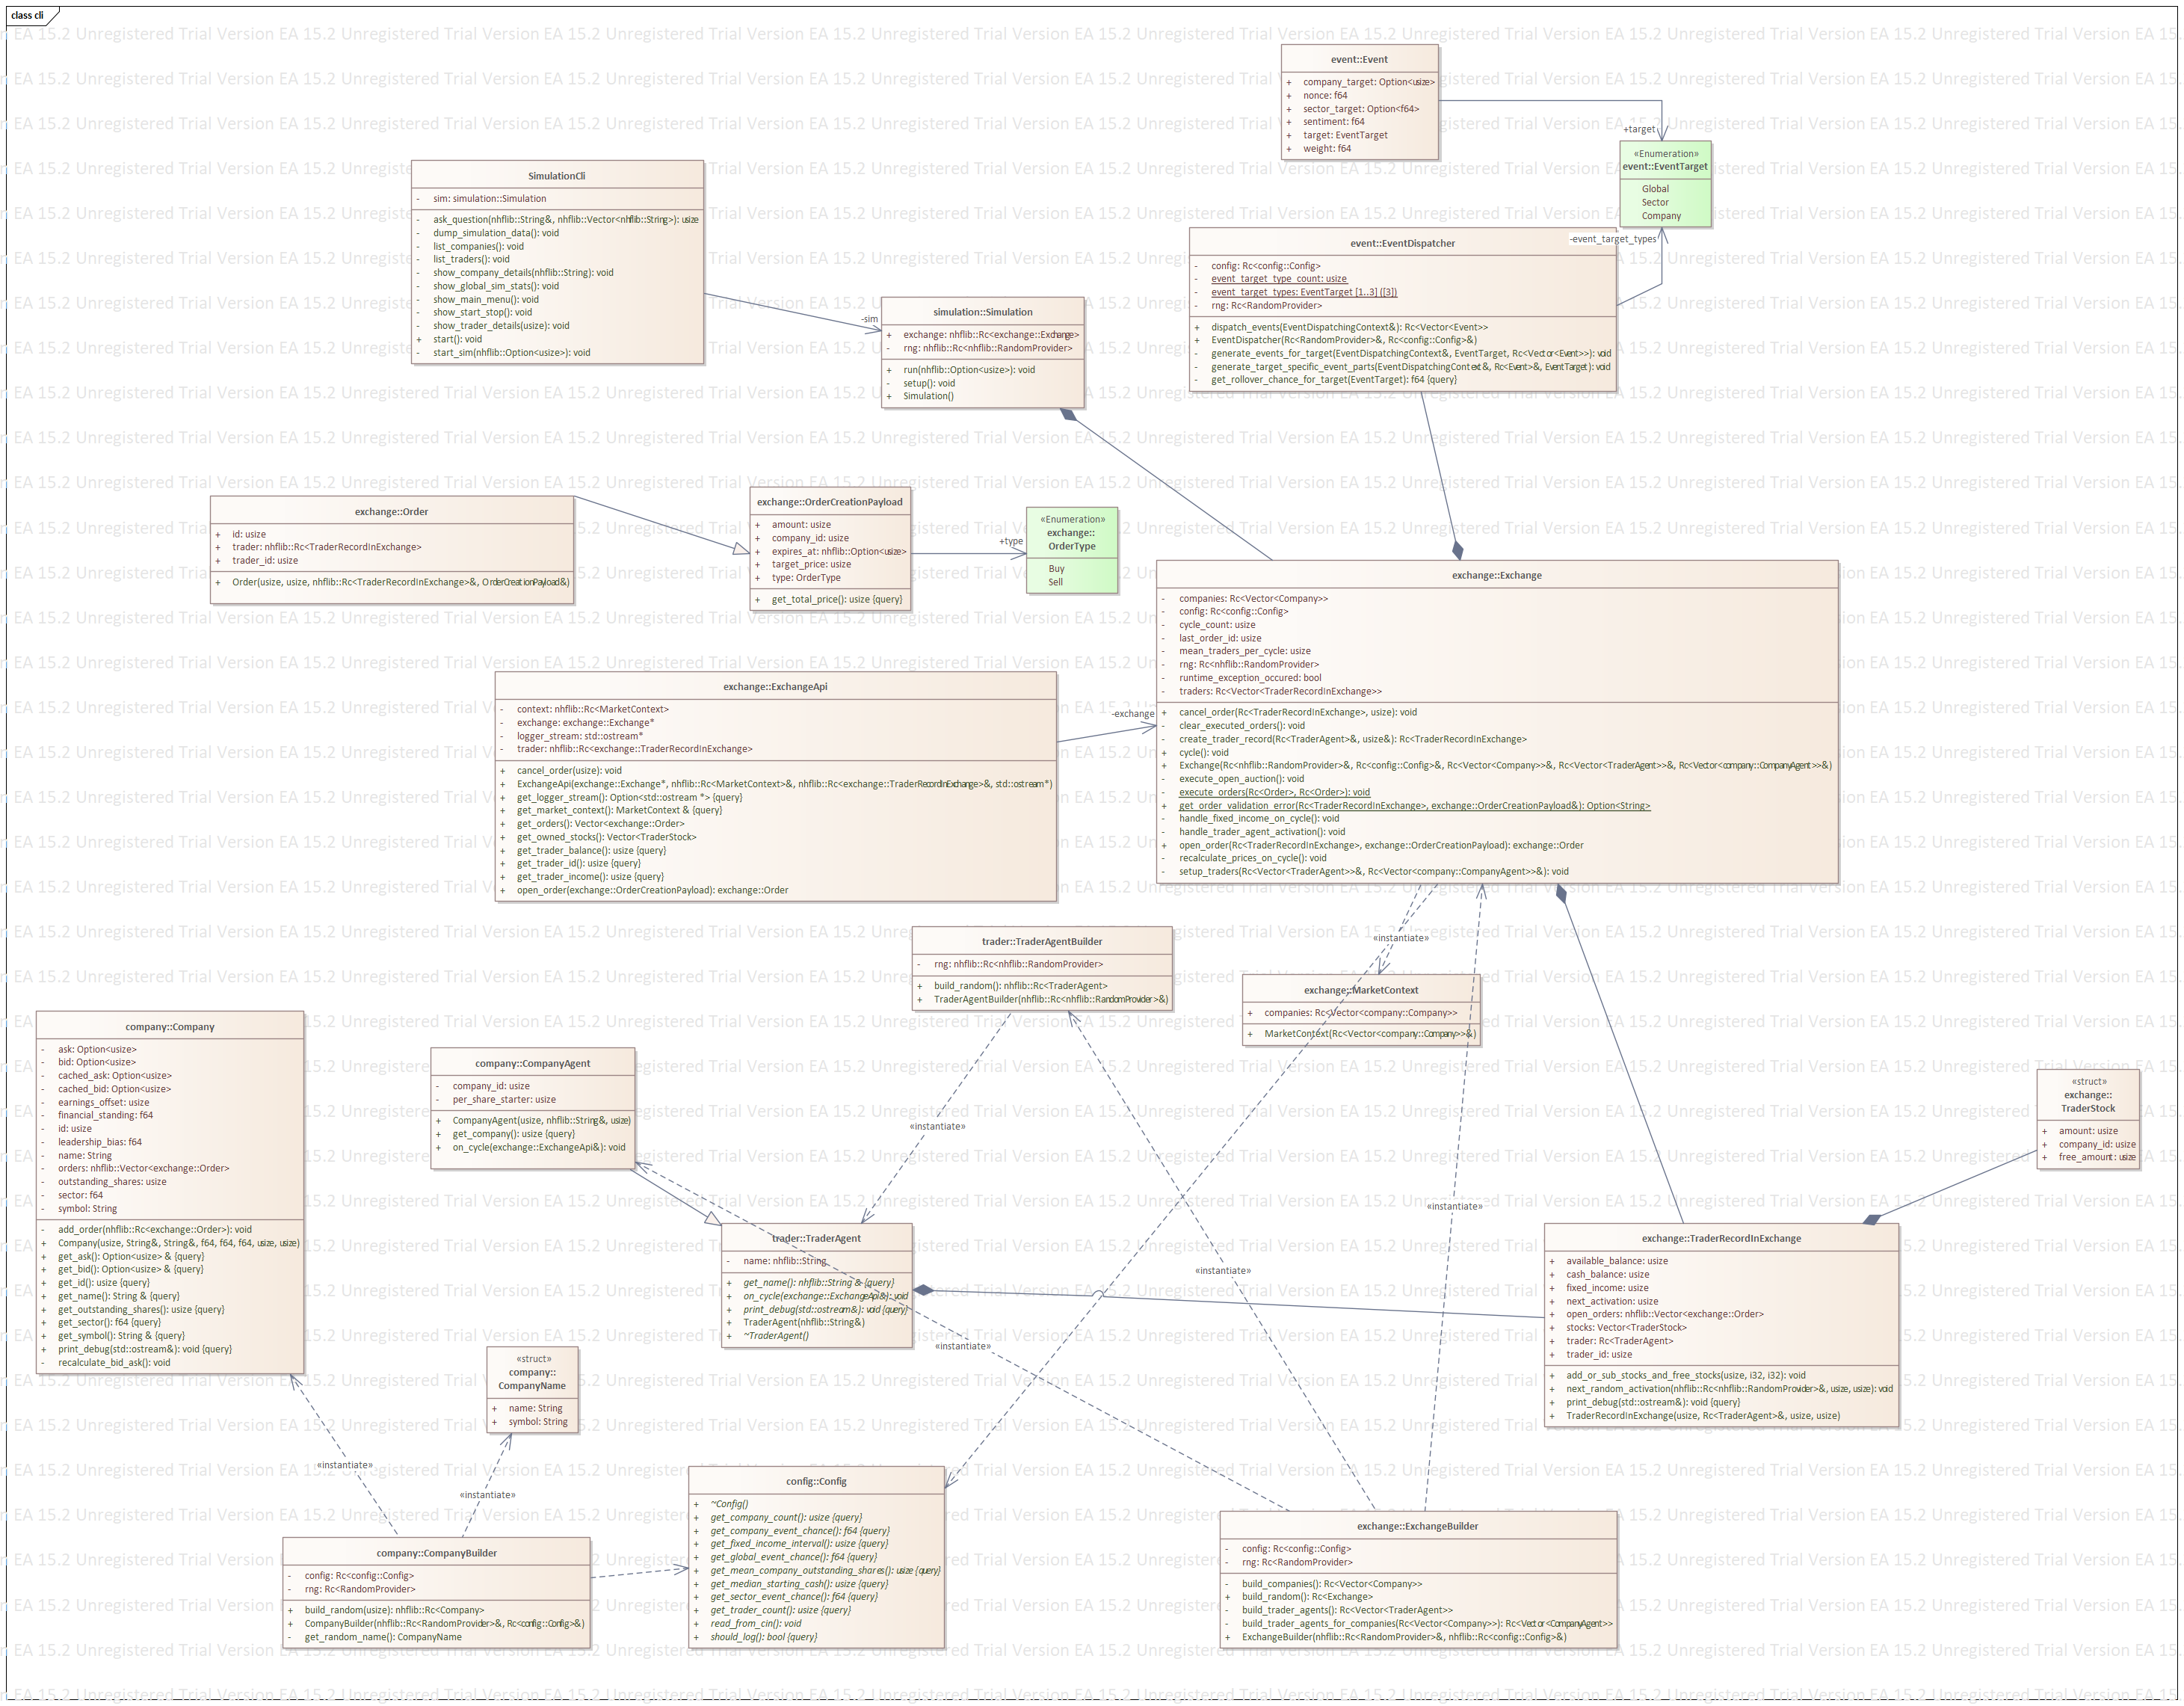
\includegraphics[scale=0.20]{cli}
    \end{center}

    \subsection{Skeleton Program Jelenlegi Állása}
    A program jelenleg előrehaladott az implementáció terén, ami még hátravan, az a kereskedői logika véglegesítése és a CLI interfész teljes lefejlesztése.
    A testprogram még hiányosságokkal rendelkezik, a piac nem minden funkciójára van teljese lefedettség.

\end{document}